\chapter{Results}
In this chapter, the performance and visual accuracy of ATLOD is 
measured.

\section{Experimental Setup}
\subsection{Hardware}
The hardware used is a MacBook Air 2020 with an Intel CPU.
The specifications are displayed in table \ref{tbl:specs}.

\begin{table}[H]
  \begin{center}
    \begin{tabular}{ c|c }
      CPU & 1.1 GHz Dual-Core Intel Core i3\\
      \hline
      Memory & 8 GB 3733 MHz LPDDR4X\\
      \hline
      Graphics & Intel Iris Plus Graphics 1536 MB\\
      \hline
      OS & macOS Monterey Version 12.6\\
      \hline
      Resolution & $2560 \times 1600$
    \end{tabular}
  \end{center}
  \caption{The specifications of the used MacBook Air 2020.}\label{tbl:specs}
  \end{table}

\subsection{Height Data and GeoMipMapping Configuration}
The height data used is the SRTM 30m data set retrieved from OpenTopography \cite{srtm2013}. 
The heightmap file
is a $13922 \times 14140$ 16-bit greyscale PNG image converted 
from a GeoTIFF file (figure \ref{fig:results-heightmap}) and covers 
a large extent of Switzerland (excluding the Grisons) and small parts 
of Germany, France and Italy. The total area is 130 km$^2$.


\begin{figure}[H]
  \centering
  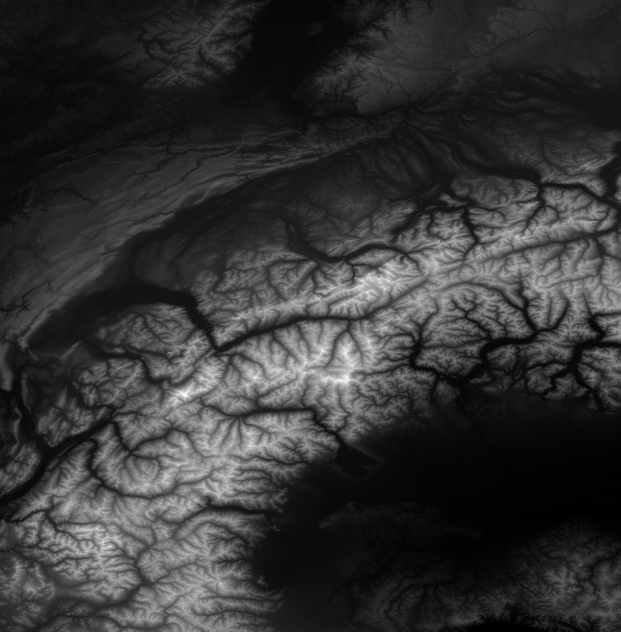
\includegraphics[width=0.7\textwidth]{results-heightmap}
  \caption{The $13922 \times 14140$ 16-bit greyscale heightmap used for benchmarking (retrieved from OpenTopography \cite{srtm2013}). In this figure, the gray values were converted from 0,\dots,65535 to 0,\dots,255 in order to make the heights more visible.}\label{fig:results-heightmap}
\end{figure}

The GeoMipMapping algorithm is configured for the best balance between 
performance and visual accuracy as shown in table \ref{tbl:bench-settings}.

\begin{table}[H]
  \begin{center}
    \begin{tabular}{ c|c }
      Block size & $2^9 + 1 = 513$\\
      \hline
      Fog factor & 0 (deactivated)\\
      \hline
      Minimum LOD & 0 (default)\\
      \hline
      Maximum LOD & 9 (default)\\
      \hline 
      Base distance & 700\\
      \hline
      LOD determination mode & Exponentially growing distance\\
      \hline
      $y$-scale & 0.03
    \end{tabular}
  \end{center}
  \caption{Rendering settings for the benchmarks.}\label{tbl:bench-settings}
  \end{table}

\subsection{Benchmarks}
Two kinds of benchmarks are performed: The \textit{performance benchmark},
which measures the framerate of rendering, and the \textit{visual accuracy benchmark}, 
which measures the image difference between GeoMipMapping and naive rendering.
For both benchmarks, no fog and no overlay texture is rendered.

For the performance benchmark, two kinds of scenarios are performed:
\begin{itemize}
  \item The first scenario is the flyover from the bottom-left corner to the top-right, whilst the camera is looking down a certain angle.
        The $y$-coordinate and the front vector of the camera are fixed during this flyover.
  \item The second scenario is the $360^{\circ}$ rotation while stationary. 
\end{itemize}

For the visual accuracy benchmark, two kinds of scenarios are performed as well:
\begin{itemize}
  \item The first scenario is a screenshot of a large section of the terrain at a great distance, once with LOD and once at full resolution.
  \item The second scenario is a screenshot of a smaller section of terrain but with a high camera zoom, once with LOD and once without.
\end{itemize}

\section{Performance Benchmarks}
The performance accuracy is computed by calculating the average FPS from the beginning of the flight 
or rotation to the end. The performance measurements of the naive renderer is not documented in this report,
but was consistently around less than 1 FPS in both scenarios.

\subsection{Flyover from Corner to Corner}
Five flyovers were conducted from the bottom-left corner to the top-right corner with various 
velocities. Table \ref{tbl:results-fps-fly} shows the FPS for each of the flyovers.

\begin{table}[H]
  \begin{center}
    \begin{tabular}{ c|c|c|c|c|c|c }
      & Flyover 1 & Flyover 2 & Flyover 3 & Flyover 4 & Flyover 5 & Average\\
      \hline
      FPS & 59.83 & 60.14 & 60.35 & 60.08 & 57.89 & 59.65
    \end{tabular}
  \end{center}
  \caption{RMSE of the large terrain screenshots 1 to 5.}\label{tbl:results-fps-fly}
\end{table}

\subsection{360\textdegree~Rotation}
Five rotations were conducted with various 
velocities. Table \ref{tbl:results-fps-rotations} shows the FPS for each of the rotations.

\begin{table}[H]
  \begin{center}
    \begin{tabular}{ c|c|c|c|c|c|c }
      & Rotation 1 & Rotation 2 & Rotation 3 & Rotation 4 & Rotation 5 & Average\\
      \hline
      FPS & 60.61 & 60.57 & 61.62 & 60.08 & 61.11 & 60.65
    \end{tabular}
  \end{center}
  \caption{RMSE of the large terrain screenshots 1 to 5.}\label{tbl:results-fps-rotations}
\end{table}

\section{Visual Accuracy Benchmarks}
For the visual accuracy benchmarks, the \textit{root mean square error (RMSE)} of 
both images is computed :
\begin{align*}
  RMSE = \sqrt{\frac{1}{mn} \sum_{x=1}^m \sum_{y=1}^n (A(x,y) - B(x,y))^2},
\end{align*}
where $m$ is the length of both images, $n$ is the height of both images and $A,B$ is the first and second image respectively \cite[p.~47]{cpvripai}.
The image difference and the RMSE are both computed using \textsc{Matlab}.

Appendix B contains all screenshots for the visual accuracy benchmarks.

\subsection{Large Terrain Screenshots}
Five screenshots of the terrain were captured at various camera positions and angles,
such that a large portion of the terrain was visible.
The RMSE of every screenshot was computed, as shown in table \ref{tbl:results-rmse-large}.

\begin{table}[H]
  \begin{center}
    \begin{tabular}{ c|c|c|c|c|c|c }
      & S. 1 & S. 2 & S. 3 & S. 4 & S. 5 & Average\\
      \hline
      RMSE & 3.94 & 3.1 & 2.59 & 1.96 & 2.32 & 2.78
    \end{tabular}
  \end{center}
  \caption{RMSE of the large terrain screenshots 1 to 5.}\label{tbl:results-rmse-large}
\end{table}

\subsection{Low FOV Screenshots}
Five screenshots of the terrain were captured at various camera positions and angles,
such that only a small portion far away was visible due to the low FOV.
The RMSE of every screenshot was computed, as shown in table \ref{tbl:results-rmse-large}.
\begin{table}[H]
  \begin{center}
    \begin{tabular}{ c|c|c|c|c|c|c }
      & S. 1 & S. 2 & S. 3 & S. 4 & S. 5 & Average\\
      \hline
      RMSE & 4.82 & 5.71 & 4.78 & 5.3 & 4.49 & 5.02
    \end{tabular}
  \end{center}
  \caption{RMSE of the low FOV screenshots 1 to 5.}\label{tbl:results-rmse-low-fov}
\end{table}

\section{Memory Consumption}
In most cases, the RAM and GPU memory consumption can be calculated manually for a given
terrain size and block size.

\subsection{RAM}
The RAM consumption is mostly dependent on how many blocks (i.e. \\ \texttt{GeoMipMappingBlock} instances) need to be managed.
Generally, the larger the block size and the smaller the terrain size, the fewer blocks need to be managed.

\subsection{GPU Memory}
The main bottleneck of this implementation in terms of GPU memory is 
the heightmap texture, which takes up 2 bytes per height value.
An alternative approach would be to support 1-byte grayscale heightmaps. However, this would 
limit the number of possible height values to 256 and therefore produce
``blocky'' looking terrain.

Memory consumption by the vertices and indices is quite low.
The number of vertices that are loaded on the GPU is only $blockSize \times blockSize$.

\subsection{Examples}
Table \ref{tbl:memory-vbo-ebo} shows the GPU memory usage by the vertex buffers and index buffers for 
various block sizes. The size of the vertex buffer was calculated with $blockSize \times blockSize \times 2 \times 4$
and size of the index buffer was computed and printed directly in ATLOD.

\begin{table}[H]
  \begin{center}
    \begin{tabular}{ c|c|c|c }
      Block size & Vertex buffer & Index buffer & Total\\
      \hline
      65 & 0.03 MB & 0.12 MB & 0.15 MB\\
      \hline 
      129 & 0.13 MB & 0.33 MB & 0.46 MB\\
      \hline
      257 & 0.52 MB & 1.02 MB & 1.54 MB\\
      \hline
      513 & 2.1 MB & 3.43 MB & 5.53 MB
    \end{tabular}
  \end{center}
  \caption{Memory consumption by the vertex and index buffers for different block sizes.}\label{tbl:memory-vbo-ebo}
\end{table}

Table \ref{tbl:memory-heightmap} shows the GPU memory usage by the heightmap texture image 
for various heightmap sizes, calculated with $heightmapSize \times heightmapSize \times 2$.

\begin{table}[H]
  \begin{center}
    \begin{tabular}{ c|c }
      Terrain size & Heightmap texture \\
      \hline
      $2000 \times 2000$ & 8 MB\\
      \hline
      $5000 \times 5000$ & 50 MB\\
      \hline
      $16000 \times 16000$ & 512 MB
    \end{tabular}
  \end{center}
  \caption{Memory consumption by the heightmap texture on the GPU for various heightmap sizes.}\label{tbl:memory-heightmap}
\end{table}

Table \ref{tbl:memory-blocks} shows the memory usage by the blocks in GeoMipMapping's block list for 
various heightmap sizes and block sizes,
calculated and printed in ATLOD direclty by multiplying the size of the list and \texttt{sizeof(GeoMipMappingBlock)}.

\begin{table}[H]
  \begin{center}
    \begin{tabular}{ c|c|c|c }
      Block size & \multicolumn{3}{|c}{Heightmap size}  \\
      \hline
      & $2000 \times 2000$ & $5000 \times 5000$ & $16000 \times 16000$\\
      \hline
      65 & 0.08 MB & 0.53 MB & 5.45 MB\\
      \hline
      129 & 0.02 MB & 0.13 MB & 1.35 MB\\
      \hline
      257 & 4.31 KB & 0.03 MB & 0.33 MB\\
      \hline
      513 & 0.79 KB & 7.12 KB & 0.08 MB\\
    \end{tabular}
  \end{center}
  \caption{Memory consumption by the block list at different block sizes and heightmap sizes.}\label{tbl:memory-blocks}
\end{table}
